\chapter{Ocean-atmosphere vertical column modelling}
\label{ch:airseaSCM}
\minitoc
We present in this chapter the concepts and equations in
the continuous level which
we will use in the rest of this thesis.
In particular, in Section \ref{sec:airseaSCM_primitiveEquations}
the primitive equations driving the circulation inside
the ocean and atmosphere are derived then
the turbulent features are described in Section
\ref{sec:airseaSCM_turbulence}.
Finally, the models used in this thesis are summed up
in Section \ref{sec:airseaSCM_hierarchy}
before discussing about Schwarz methods in Section
\ref{sec:airseaSCM_Schwarz}.
\section{Derivation of the primitive equations}
\label{sec:airseaSCM_primitiveEquations}
This section aims to present the so-called
primitive equations, which are used to model
the inner parts of both the atmosphere and ocean.
\subsection{Non-turbulent primitive equations}
We start from the Navier-Stokes momentum equation in a rotating frame:
\begin{equation}
\label{eq:airseaSCM_momentumNavierStokes}
\rho \left(\partial_t + \mathbf{U} \cdot \nabla \right) \mathbf{U}
= - \nabla p + K_{u, {\rm mol}} \Delta \mathbf{U} - \rho \mathbf{g}
- 2 \mathbf{\Omega} \times (\rho \mathbf{U})
\end{equation}
where the symbols are given in Table
\ref{tab:airseaSCM_primitiveEquationsSymbols}
\begin{table}
\centering
\begin{tabular}{c|c|c}
Symbol & Quantity & Unit \\
\hline
$\rho$& {Density} & ${\rm kg}.{\rm m}^{-3}$ \\
$p$   & {Pressure} & ${\rm kg}.{\rm m}^{-1}.{\rm s}^{-2}$ \\
$\mathbf{U}$ & {Velocity}& ${\rm m}.{\rm s}^{-1}$ \\
$\theta$ & {Potential temperature}& ${\rm K}$ \\
$K_{u, {\rm mol}}$ & {Molecular viscosity}& ${\rm m}^{-1}.{\rm s}^{-2}$ \\
$\mathbf{g}$ & {Gravity acceleration}& ${\rm kg}.{\rm m}.{\rm s}^{-2}$ \\
$\mathbf{\Omega}$ & {Angular speed}& ${\rm rad}.{\rm s}^{-1}$ \\
$\nabla$ & {Spatial Gradient} & ${\rm m}^{-1}$\\
$\Delta$ & {Spatial Laplacian} &${\rm m}^{-2}$
\end{tabular}
\caption{Symbols used in Section
\ref{sec:airseaSCM_primitiveEquations}. Bold letters
indicate that the quantity lies in $\mathbb{R}^3$.}
\label{tab:airseaSCM_primitiveEquationsSymbols}
\end{table}
and the \textit{continuity equation} which ensures
conservation of mass:
\begin{equation}
\label{eq:airseaSCM_conservationMass}
\partial_t \rho = - \nabla \cdot (\rho \mathbf{U})
\end{equation}
\myTD{J'ai paraphrasé la thèse de Sophie dans l'itemize}
It is now possible to simplify the two equations
\eqref{eq:airseaSCM_momentumNavierStokes} and
\eqref{eq:airseaSCM_conservationMass} with
some usual approximations:
\begin{itemize}
\item \textit{Spherical geoid approximation}:
we assume that the earth is spherical and that the
gravity acceleration is given by
$\mathbf{g} =\begin{pmatrix}
0\\ 0 \\ g
\end{pmatrix}$ where $g=9.81 {\rm m}.{\rm s}^{-2}$.
\item \textit{Traditional approximation}:
We neglect the horizontal terms of
$\mathbf{\Omega}$: we assume that
$\mathbf{\Omega} =\begin{pmatrix}
0\\ 0 \\ f/2
\end{pmatrix}$ where $f$ depends on the latitude.
\item \textit{Hydrostatic fluid}:
the pressure gradient balances the gravity force:
$\partial_z p = -\rho g$. We neglect the vertical
acceleration due to pressure and gravity.
This approximation is usually done for large time
scales like the one used in climate simulations.
\item \textit{Boussinesq approximation}
\citep{boussinesq_theorie_1903}:
the density $\rho$ is close to a constant $\rho_0$.
The variation of density $\widetilde{\rho} =
\rho - \rho_0$ is neglected except when computing
the pressure gradient $\partial_z p = - \rho g$.
The atmosphere models rely on compressibility and
do not use this approximation. However, we make
the Boussinesq approximation for both domains
as we assume that the compressibility effects
are small close to the surface and that they
can be neglected to study the surface layer.
\end{itemize}
We hence obtain the \textit{non-turbulent}
primitive equations:
\begin{equation}
	\label{eq:airseaSCM_nonTurbulentPrimitiveEq}
\begin{cases}
	\nabla \cdot \mathbf{U} &= 0 \\
	\partial_t u + \nabla \cdot (\mathbf{U} u) &=
	- \frac{\partial_x p}{\rho_0} + K_{u, {\rm mol}} \Delta u
	+ f v \\
	\partial_t v + \nabla \cdot (\mathbf{U} v) &=
	- \frac{\partial_y p}{\rho_0} + K_{u, {\rm mol}} \Delta v
	- f u \\
	\partial_z p &= -\rho g
\end{cases}
\end{equation}
where we noted $\mathbf{U} = \begin{pmatrix}u\\v\\w\end{pmatrix}$.
\paragraph{Stratification}
$\rho$ is given by an equation of state, which only involves
the temperature in our case (in particular, the effect
of humidity (in the atmosphere) and salinity (in the ocean)
are neglected):
A \textit{neutral} stratification refers to a constant 
density along the vertical axis. Since the density is
constant, the temperature does not need to be computed
to integrate in time the wind speed.
\par
On the contrary, in a \textit{stratified} case the
density depends on the potential temperature $\theta$:
\begin{equation}
	\rho = \rho_{\rm eos}(\theta), ~~~~~~~~~~~
	\partial_t \theta + \nabla \cdot (\mathbf{U} \theta) =
	K_{\theta, {\rm mol}} \Delta \theta + F_\theta
\end{equation}
where $K_{\theta, {\rm mol}}$ and $F_\theta$ are
the molecular diffusivity and some forcing term.
$\theta$ must be computed jointly with the wind
speed to solve the system
\eqref{eq:airseaSCM_nonTurbulentPrimitiveEq}.

\subsection{Reynolds decomposition}
The solution of the system \eqref{eq:airseaSCM_nonTurbulentPrimitiveEq}
contains very small scales which cannot be solved numerically for
large domains such as the ocean or the atmosphere. It is hence usual
to use the \textit{Reynolds decomposition}, which consists in
separatinig the variables into an "average" part which can be
represented by the numerical schemes and a fluctuating part which
will be parameterized with turbulent closure schemes
(detailed later in \S \ref{sec:airseaSCM_turbulentClosure}).
\par
For $X=u, v, w, p$ or $\theta$, we note
\begin{equation}
	X = \langle X\rangle + X'
\end{equation}
where $\langle \cdot \rangle$ represents a \textit{statistical}
average which satisfies:
\begin{equation}
\begin{aligned}
	\langle X' \rangle &= 0 \\
	\langle \partial_\beta X \rangle &=
	\partial_\beta \langle  X \rangle, ~~~\beta=x,y,z,t \\
	\langle\langle \cdot \rangle\rangle &= \langle \cdot \rangle \\
	\langle \langle X \rangle Y\rangle &= \langle X \rangle\langle Y \rangle
\end{aligned}
\end{equation}
using those properties, the Reynolds decomposition of 
\eqref{eq:airseaSCM_nonTurbulentPrimitiveEq} gives:
\begin{equation}
	\label{eq:airseaSCM_TurbulentPrimitiveEq}
\begin{cases}
	\nabla \cdot \langle\mathbf{U}\rangle &= 0 \\
	\partial_t \langle u \rangle+ \nabla \cdot
	(\langle\mathbf{U}\rangle \langle u\rangle) &=
	- \frac{\partial_x \langle p\rangle}{\rho_0} +
	K_{u, {\rm mol}} \Delta \langle u\rangle
	+ f \langle v\rangle - \nabla \cdot \langle
	\mathbf{U}' u'\rangle\\
	\partial_t \langle v\rangle + \nabla \cdot
	(\langle \mathbf{U}\rangle \langle v\rangle) &=
	- \frac{\partial_y \langle p\rangle}{\rho_0} +
	K_{u, {\rm mol}} \Delta \langle v\rangle
	- f \langle u\rangle  - \nabla \cdot \langle
	\mathbf{U}' v'\rangle\\
	\partial_z\langle p\rangle &= -\rho g \\
	\partial_t \langle\theta\rangle + \nabla \cdot
	(\langle\mathbf{U}\rangle \langle\theta\rangle) &=
	K_{\theta, {\rm mol}} \Delta \langle\theta\rangle
	+ F_\theta - \nabla \cdot \langle
	\mathbf{U}' \theta'\rangle\\
	\rho &= \rho_{\rm eos}(\langle\theta\rangle)
\end{cases}
\end{equation}
From now on, this thesis will only focus the vertical terms
$\langle w' u'\rangle$, $\langle w' v'\rangle$ and
$\langle w' \theta'\rangle$
because the surface layer turbulent features are mainly limited
to those terms. For the same reason, we restrict our spatial
domain to one dimension: the equations modelize a vertical column
of atmosphere and of ocean.
The vertical speed $w$ can be eventually recovered with the
equation $\nabla \cdot \langle\mathbf{U}\rangle = 0$
but we will not directly simulate it and examine only
$\langle u \rangle, \langle v \rangle$ and $\langle \theta \rangle$.
Finally, note that \eqref{eq:airseaSCM_TurbulentPrimitiveEq}
is completed with boundary conditions that we omitted:
they will be given for our models of interest in
\S\ref{sec:airseaSCM_WallLaw}.
\par
With this decomposition we obtain more unknown than
equations because of the introduction of the terms
$\langle w' u'\rangle, \langle w' v'\rangle$
and $\langle w' \theta'\rangle$:
this is known as the turbulent closure problem.
\section{The turbulence}
\label{sec:airseaSCM_turbulence}
To tackle the turbulent closure problem,
we now provide additional relations between
the turbulent terms
$\langle w' u'\rangle, \langle w' v'\rangle,
\langle w' \theta'\rangle$ and the average quantities
$\langle u\rangle, \langle v\rangle, \langle \theta \rangle,
\langle p \rangle$.
We first detail a common choice of parameterization
for the turbulent closure far from the surface and then
(in \S\ref{sec:airseaSCM_WallLaw}) focus on the surface layer
which acts as a bottom boundary condition for
\eqref{eq:airseaSCM_TurbulentPrimitiveEq} in the atmosphere.
The ocean case is discussed in \S\ref{sec:airseaSCM_twoSided}.
\subsection{Turbulent closure and kinetic energy}
\label{sec:airseaSCM_turbulentClosure}
\paragraph{Boussinesq hypothesis}
From the observation that the turbulent term acts like a diffusion
term oriented "down-gradient", the turbulent terms are approximated
with the help of a "turbulent viscosity" $K_u$ and a
"turbulent diffusivity" $K_\theta$:
\begin{equation}
\langle w' u'\rangle = - K_u \partial_z \langle u \rangle, ~~~
\langle w' v'\rangle = - K_u \partial_z \langle v \rangle, ~~~
\langle w' \theta'\rangle =
	- K_\theta \partial_z \langle \theta \rangle
\end{equation}
This is known as the \textit{Boussinesq hypothesis}
(\citep{boussinesq_theorie_1897},
different from the Boussinesq \textit{approximation} neglecting
effects of compressibility)
The turbulent viscosity can be defined in a lot of different ways.
A typical formulation for $K_u, K_\theta$ is
\begin{equation}
	K_u = C_m l_m \sqrt{e}, ~~~~~~~ K_\theta = \frac{C_s}{\rm Pr}
	l_m \sqrt{e}
\end{equation}
where $C_m, C_s$ are constants; ${\rm Pr}$ is the so-called turbulent
Prandtl number; the mixing length $l_m$ is a characteristic
length of the turbulent flow and depends on the stratification.
$e$ is an important quantity often used in the models,
the Turbulent Kinetic Energy (TKE):
\begin{equation}
	e = \frac{1}{2} \left(\langle (u')^2 \rangle + \langle (v')^2 \rangle
	+ \langle (w')^2 \rangle\right)
\end{equation}
The evolution equation for the TKE is
\begin{equation}
	\partial_t e - 
\underbrace{\partial_z \left(K_e
    \partial_z e\right)}_{\text{diffusion with } K_e \propto K_u}
    = P + B - \epsilon
\end{equation}
where $P>0$ and $B$ are terms denoting respectively
the shear and buoyancy production of kinetic energy;
$\epsilon>0$ is the dissipation rate of TKE
into heat.
\par
$P$ corresponds to the energy lost by $\langle u \rangle$ by the
\textit{shear} term
$\partial_z \left(K_u \partial_z \langle u \rangle\right)$:
to compute it, we multiply by $\langle u \rangle$ the equation
$\partial_t \langle u \rangle = \partial_z (K_u \partial_z \langle u \rangle)$
and express the result as a function of the
energy of the mean velocity $\frac{\langle u \rangle^2}{2}$.
This gives (e.g. \citep{burchard_energy-conserving_2002},
where the derivation is done in the continuous and in the
discrete level.)
\begin{equation}
	\partial_t \left(\frac{\langle u \rangle^2}{2}\right)
	- \partial_z \left(K_u
	\partial_z\left(\frac{\langle u \rangle^2}{2}\right)\right)
	= - K_u\left(\partial_z \langle u \rangle\right)^2
\end{equation}
where $P=K_u \left(\left(\partial_z \langle u \rangle\right)^2 +
\left(\partial_z \langle v \rangle\right)^2\right)$ is the energy
\textit{produced} by the shear.
\par
A similar treatment with the density
(whose diffusion term is multiplied by $z$ instead of $\langle u \rangle$)
gives that the potential energy
is increased or reduced by $B = -K_\theta N^2$ where
$N^2 = - \frac{g\partial_z \rho}{\rho_0}$ is the Brunt-Väisälä
frequency.
The dissipation rate $\epsilon$ can be parameterized by
$\epsilon \propto \frac{e^{3/2}}{l_{\epsilon}(z)}$
where $l_\epsilon$ is a mixing length similar to $l_m$.
This parameterization of $\epsilon$ gives the widely used
\textit{Prandtl's one-equation turbulence model}.
\par
Finally, the one-dimensional evolution equation for the TKE is
\begin{equation}
\label{eq:airseaSCM_TKE_evolution}
    \begin{aligned}
    \partial_t e =
    \underbrace{\partial_z \left(K_e
    \partial_z e\right)}_{\text{diffusion}}
	    + \underbrace{K_u \left(\left(\partial_z
	    \langle u \rangle\right)^2 +
	    \left(\partial_z \langle v \rangle\right)^2\right)
	    }_{\text{shear}} 
    - \underbrace{K_{\theta} N^2 }_{\text{buoyancy}}
    - \underbrace{c_{\epsilon}
    \frac{e^{3/2}}{l_{\epsilon}(z)}}_{\text{dissipation}}
    \end{aligned}
\end{equation}
\subsection{Law of the wall and Monin-Obukhov Similarity Theory}
\label{sec:airseaSCM_WallLaw}
% 
% Pour l'hypothèse de surface libre: c'est en fait une conséquence
% de négliger l'humitidé. L'océan ne change pas de volume
% 
% C'est une hypothèse qui est faite en pratique de considérer l'océan comme ayant une géométrie plane.
% Même ayant une surface libre dans l'océan, l'atmosphère le voit comme une surface plane
% Mais en 1D la question se pose pas.
% Du coup on peut ptet l'enlever du chap1
% 
% In all this thesis, we will assume that the water
% surface is flat: this restriction strongly simplifies
% the column models, in particular when the space step becomes
% smaller than the surface waves.
% The free ocean surface is beyond the scope of this thesis:
% however, excluding explicitly
% the surface layer from the computational
% domain (like it will be done in Chapters \ref{ch:ND},
% \ref{ch:OceanND}) may lead to
% a relatively simple handling of the free surface.
We call \textit{surface layer} the area close to the ocean surface
such that it responds to a change at the surface with a short
timescale\footnote{In the litterature, a boundary layer can also
be defined as the region in which the fluid goes from zero
velocity to the maximum velocity: this definition is however
less adapted to the oceanic surface layer where the currents
are driven by the surface wind.}.
Wall modelling gives us a description of the surface layer
and provides the boundary conditions for
$\langle w' u'\rangle, \langle w' v'\rangle$ and
$\langle w' \theta'\rangle$.
The turbulence characterization of \S \ref{sec:airseaSCM_turbulentClosure}
is not accurate in the neighborhood of the interface.
\myTD{transition}
\par
For the atmosphere, the ocean surface can be seen as a
rough surface : the wind cannot slip on the ocean which
means that the velocity of the wind is zero
relatively to the surface.
\par
\myTD{copié-collé du chapitre 4:}
\par
In fluid dynamics, the presence of a rough surface makes strong
gradients appear:
due to the no-slip boundary condition
the scales of motion close to the surface are much smaller than
elsewhere in the domain and it is numerically
intractable in most applications
to refine the mesh enough for those small scales.
The models hence exclude from the computational domain
a part of the surface layer, using an adapted boundary
condition.
%
\paragraph{Neutral case}
We first present the case without stratification:
\citep{karman_mechanische_1930} noticed that the
fluids close to rough surfaces present similarities and
propose a universal function based on dimensional analysis.
Von Kàrmàn also states that "the characteristic length
of the flow pattern is proportional to
[the distance to the wall]".
\par
We list below the main features of the surface layer:
\begin{itemize}
	\item the Coriolis effect and the geostrophic forcing are
		neglected (we assume that the effect of the
		proximity to the surface is predominant);
	\item it is well mixed: the governing equation
		is quasi-stationary (the surface layer
		immediately adjusts to the external parameters).
		As a consequence, the flux $K_u \partial_z u$
		is a constant along the vertical axis.
	\item The vertical profile of $K$ strongly depends 
		on $z$.
		The size of the turbulent eddies at height $z$
		is proportional to the distance to the surface $z$
		(e.g. \cite{kawai_wall-modeling_2012}, see Figure
		\ref{fig:airseaSCM_eddiesDrawing}).
		As a consequence, the turbulent viscosity
		linearly scales with $z+z_u$:
		\begin{equation}
			K_u \propto z+z_u
		\end{equation}
		where $z_u$ accounts for both the molecular
		viscosity and the geometry of the surface.
		We also have for the turbulent diffusivity
		$K_\theta \propto z+z_\theta$.
\end{itemize}
We now interest ourselves into the horizontal component of
the speed. We first assume that it is aligned with the
direction of $u$: since the Coriolis effect
is neglected and the turbulence is assumed isotropic,
there is no rotation of the fluid inside the surface layer
and we can assume that $v=0$
with a rotation of the axis reference.
We will use the orientation of the wind speed later.
\par
Let us define \textit{friction scales} $u_\star$
, $z_{u}$ such that $u_\star^2 =
|\langle w' u' \rangle|$ and
$z_{u} = z_{u}(K_{\rm mol}, u_\star)$
(see e.g. \citep{schlichting_boundary_1960}
for the choice of $z_{u}$ as a constant
of integration).
\begin{figure}
	\centering
	\subimport{images/}{EddiesDrawing.pdf_tex}
	\caption{The characteristic size of the eddies
	(in purple) is proportional to the distance to the
	surface. The link between the size of the eddies
	and the logarithmic profile (in orange) is
	the constant flux approximation.
	}
	\label{fig:airseaSCM_eddiesDrawing}
\end{figure}
The law of the wall reads
\begin{equation}
	\label{eq:airseaSCM_LawOfWallProfile}
	u(z) - u(0) = \frac{u_\star}{\kappa} \ln(\frac{z+z_u}{z_u})
\end{equation}
where $\kappa = 0.4$ is the Von Kàrmàn constant.
\begin{remark}
	Generally, the law of the wall
	refers to an expression using
	$\ln(\frac{z}{z_u})$. By using $z+z_u$
	instead of $z$,
	the molecular sub-layer is included
	inside the law of the wall: we can hence
	use the profile of $u$ for small $z$
	\citep{pelletier_two-sided_2021}.
	This formulation is not standard but it is
	appropriate for mathematical analyses and
	it does not change the results
	significantly.
\end{remark}
\paragraph{Stratified case}
The extension of the law of the wall to stratified
fluids is called \textit{Monin-Obukhov Similarity Theory}.
It is used in all ocean-atmosphere couplings to our knowledge.
The quasi-stationarity is also assumed for the temperature
and $K_u \partial_z u$ and $K_\theta \partial_z \theta$
are both constants along the vertical axis.
We can define a friction scale $\theta_\star$
for the potential temperature, such that
\begin{equation}
	\langle w' \theta' \rangle = u_\star \theta_\star
\end{equation}
To describe the stratification, the \textit{Obukhov length}
is used:
\begin{equation}
	L_{MO} = \frac{u_\star^3}{g \kappa
	\frac{\theta_\star}{\theta(\delta_{sl})}}
\end{equation}
which is the only characteristic length describing
accurately the effect of the stratification in
the surface layer \citep{obukhov_turbulence_1946}.
$L_{MO}>0$ in stable stratifications
(where $\theta_\star>0$)
and $L_{MO}<0$ in unstable stratifications
(where $\theta_\star>0$).
The neutral case will be recovered
for $L_{MO} \rightarrow \infty$, corresponding
to $\theta_\star \rightarrow 0$.
\par
The difference with the neutral case is then contained
in \text{stability functions} $\phi_m, \phi_h$:
\begin{equation}
\begin{aligned}
	K_u &\propto (z+z_u)~ \phi_m(\frac{z}{L_{MO}}) \\
	K_\theta &\propto (z+z_u)~ \phi_h(\frac{z}{L_{MO}})
\end{aligned}
\end{equation}
Typical stability functions are plotted in the left panel of Figure
\ref{fig:airseaSCM_stabilityfunctions}.
A stable (resp. instable) stratification leads to a
decrease (resp. increase) of $K_u, K_\theta$ and
$L_{MO}\rightarrow \infty$ recovers the neutral case.
\begin{figure}
	\centering
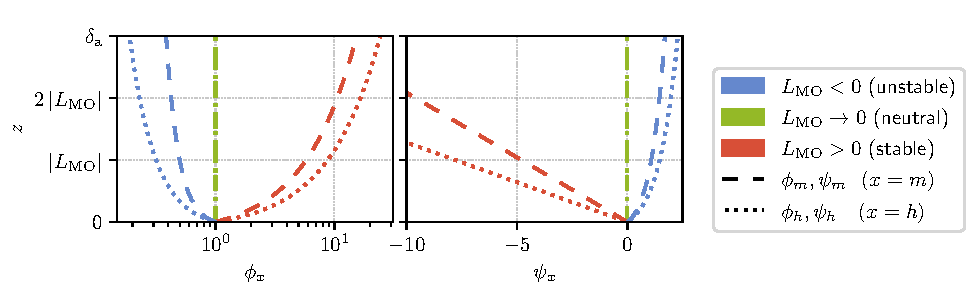
\includegraphics[scale=0.8]{images/stabilityfunctions.pdf}
	\caption{Typical profiles of the stability functions (left)
	and of their integrated form (right) in the
	surface layer $[0,\delta_{\rm sl}]$. In the unstable
	and stable cases, $\frac{\delta_{\rm sl}}{L_{\rm MO}}$
	was set to respectively -3 and 3.
	}
	\label{fig:airseaSCM_stabilityfunctions}
\end{figure}
To obtain the solution profiles,
the \textit{integrated forms}
of the stability functions $\psi_m, \psi_h$
are defined as
\begin{equation}
	\psi_x \left(\frac{z}{L_{MO}}\right)
	= \int_0^{\frac{z}{L_{MO}}}
	\frac{1 - \phi_x(\zeta)}{\zeta} d\zeta
	, ~~~~x=m,h
\end{equation}
and we have
\begin{equation}
\label{eq:airseaSCM_MOSTprofiles}
\begin{aligned}
	||u(z)-u(0)|| = \frac{u_\star}{\kappa}
    \left(
	\ln(1+\frac{z}{z_{u}})
	\emphase{- \psi_m\left(\frac{z}{L_{MO}}\right)}
    \right)
    \\
    \theta(z) - \theta_s = 
	\frac{\emphase{\theta_\star}}{\kappa}
    \left(
	\ln(1+\frac{z}{z_{\theta}})
	\emphase{- \psi_h\left(\frac{z}{L_{MO}}\right)}
\right)
\end{aligned}
\end{equation}
Monin-Obukhov Similarity Theory
is extensively used (e.g. \citep{basu_cautionary_2017});
it is however not universally
accepted in particular in very stable stratifications
(see \citep{optis_moving_2014}).
\paragraph{Bulk algorithm}
Using \eqref{eq:airseaSCM_MOSTprofiles} and the values of
$u(\delta_{sl}) - u(0)$ and $\theta(\delta_{sl}) - \theta_s$
it is possible to compute the friction scales
$u_\star, \theta_\star$. It is however not trivial as
$L_{MO}$ and $z_u, z_\theta$ depend themselves on
$u_\star, \theta_\star$.
The so-called "bulk algorithm" are designed for this
task: they generally rely on a fixed-point method:
\begin{enumerate}
\item input: $u(\delta_{sl}) - u(0)$
		and $\theta(\delta_{sl}) - \theta_s$;
\item choose a first guess $u_\star^{n=0}, \theta_\star^{n=0}$;
\item iteratively apply
	\eqref{eq:airseaSCM_MOSTprofiles} (or
	\eqref{eq:airseaSCM_LawOfWallProfile} in the neutral case)
	to compute $u_\star^{n}, \theta_\star^{n}$ using
	$u_\star^{n-1}, \theta_\star^{n-1}$
	in the expressions of $z_u, z_\theta$ and $L_{MO}$;
\item at convergence ($u_\star^{n},\theta_\star^{n} \approx
	u_\star^{n-1},\theta_\star^{n-1}$) return the friction
		scales $u_\star = u_\star^{n},
		\theta_\star = \theta_\star^{n}$ (or only
		$u_\star = u_\star^{n}$ in the neutral case)
\end{enumerate}
\subsection{Two-sided bulk}
\label{sec:airseaSCM_twoSided}
The ocean and atmosphere have not been distinguished in equations
so far. From this point, we will use a subscript "o" for the ocean
quantities and "a" for the atmosphere quantities.
In Chapter \ref{ch:OceanND} we will also consider the
\textit{oceanic surface layer}.
The sea surface temperature and the surface currents are often
evaluated below the surface. The common approach is
to neglect the difference between the temperature and currents
below and at the surface. However,
some efforts have been made to correct the satellite
measurement: \citep{donlon_toward_2002} show that
the difference between
the surface temperature and the sub-surface temperature is
approximatively constant for medium and strong winds but that 
it is harder to evaluate in stratified condition corresponding
to winds slower than $6 \; {\rm m}.{\rm s}^{-1}$).
\citep{ward_near-surface_2006}
"\textit{show the strong dependency of the SST on air-sea heat
flux estimates, with warm-layer errors of almost
60 ${\rm W}.{\rm m}^{-2}$ associated with intense stratification. This indicates
the importance of the inclusion of the skin temperature for
accurate calculation of latent, sensible, and net longwave
heat fluxes}".
In \citep{pelletier_two-sided_2021} a non-standard bulk formulation
which uses Monin-Obukhov Similarity Theory (MOST) in the oceanic
surface layer is derived.
We follow this idea and incorporate to our coupled model an
oceanic surface layer which follows the same principles as
the surface layer in the atmosphere.
To satisfy the continuity of the fluxes across the interface,
the friction scales of the ocean are
$\sqrt{\frac{\rho_{\rm a}} {\rho_{\rm o}}} u_\star$ and
$\sqrt{\frac{\rho_{\rm a}}{\rho_{\rm o}}
\frac{c_{\rm a}^p}{c_{\rm o}^p}}
\theta_\star$ where $c_{\rm o}^p, c_{\rm a}^p$
are the heat capacities of water and air.
We hence have for $\delta_o \leq z \leq 0$ (where $\delta_o \leq 0$
is the depth of the surface layer):
\begin{equation}
	\begin{aligned}
	||K_u \partial_z u|| &= \frac{\rho_a}{\rho_o}
	u_\star^2\\
	||K_\theta \partial_z \theta|| &=
	\frac{\rho_{\rm a} c_{\rm a}^p}{\rho_{\rm o} c_{\rm o}^p}
	\theta_\star u_\star
	\end{aligned}
\end{equation}
and the reconstruction of $u$, $\theta$ follow equations
similar to \eqref{eq:airseaSCM_MOSTprofiles}:
\begin{equation}
\label{eq:airseaSCM_MOSTprofilesOSL}
\begin{aligned}
	||u(0)-u(z)|| = \emphase{\frac{\rho_a}{\rho_o}}
	\frac{u_\star}{\kappa}
    \left(
	\ln(1-\frac{z}{z_{u}^o})
	\emphase{- \psi_m^o\left(-\frac{z}{L_{MO}}\right)}
    \right)
    \\
	\theta_s - \theta(z) = 
	{\sqrt{\frac{\rho_{\rm a}}{\rho_{\rm o}}
	\frac{c_{\rm a}^p}{c_{\rm o}^p}}}
	\frac{{\theta_\star}}{\kappa}
    \left(
	\ln(1-\frac{z}{z_{\theta}^o})
	{- \psi_h^o\left(-\frac{z}{L_{MO}}\right)}
\right)
\end{aligned}
\end{equation}
If $\delta_o$ is set to zero, then there is no surface layer
in the ocean and we call the surface layer \textit{one-sided}.
in the other case ($\delta_o<0$) the surface layer is
\textit{two-sided}.
The full coupled problem described until here
is called "turbulent Ekman problem". It is summed up in
\S\ref{sec:airseaSCM_hierarchy_TurbulentEkman}.
\section{A hierarchy of models}
\label{sec:airseaSCM_hierarchy}
The analysis of coupling algorithms applied to the
ocean-atmosphere system requires additional
simplifications to be performed.
These simplifications form a hierarchy of models, from
the most sophisticated to the most idealized:
\begin{enumerate}
	\item \textbf{Turbulent Ekman}: described in the previous
		sections.
	\item \textbf{Ekman}: additionally,
		the viscosity is constant in the
		atmosphere and in the ocean; $u_\star$ is constant.
	\item \textbf{Reaction-diffusion}: The surface layer is ignored;
		the density jump is neglected;
		the Coriolis term is replaced by a reaction term.
\end{enumerate}
\subsection{Ekman problem Neutral or Stratified with bulk and turbulent kinetic energy}
\label{sec:airseaSCM_hierarchy_TurbulentEkman}
The \textbf{Turbulent Ekman} model is the one described up till now.
We restrict ourselves to a vertical column of atmosphere
above a vertical column of ocean.
To avoid having to carry $u, v, w$ in all the equations
the vertical speed $w$ is not explicitly represented
(it can be however deduced from $u,v$ and the equation
$\nabla \cdot \mathbf{U}=0$).
Moreover, $u$ and $v$ will be represented together in
a single complex variable $u^{\mathbb{C}} = u+iv$.
The rotation of the Coriolis effect corresponds to
a rotation in the complex plane.
Indeed, rewriting \eqref{eq:airseaSCM_TurbulentPrimitiveEq}
with an operator ${\cal L}$ corresponding to everything except
the Coriolis term gives:
\begin{equation}
	\label{eq:airseaSCM_complexForm}
\begin{cases}
	{\cal L}u &= fv\\
	{\cal L}v &= - fu = (i^2) f u
\end{cases}
\end{equation}
which can be written ${\cal L}u^{\mathbb{C}} = -i f u^\mathbb{C}$.
In the following we will drop the ${\mathbb{C}}$ exponent
and use a reaction term $ifu$ for the Coriolis effect.
\begin{figure}
	\centering
	\subimport{images/}{oneSided.pdf_tex}
	~~~~~
	\subimport{images/}{twoSided.pdf_tex}
	\caption{\textit{one-sided} surface layer
	(left) and \textit{two-sided} surface layer (right).
	\myTD{include bd cond et temperature}
	}
	\label{fig:airseaSCM_twoSidedBulk_drawing}
\end{figure}
\myTD{recap du système couplé avec temperature, neutre ou pas}
Figure \ref{fig:airseaSCM_twoSidedBulk_drawing} gives
the equations of the coupled system. In the \textit{stratified}
case, the potential temperature $\theta$ is jointly computed with the
momentum $u$ whereas in the \textit{neutral} case the momentum
is the only quantity of interest.
\subsection{Ekman problem with a friction law}
\label{sec:airseaSCM_hierarchy_Ekman}
The discrete analysis of the convergence of Schwarz methods
requires a constant viscosity. This is a very strong assumption
which leads to a vertical mixing not physically relevant.
However, it allows to study the effect of the surface layer on the
convergence of Schwarz methods.
The bulk methods used to parameterize the surface layer use
implicitly defined applications which are hard to deal with
in a convergence study. For this reason, we also assume
that $u_\star$ is constant but we keep a proximity with
the usual parameterizations of the surface layer
by formulating $u_\star^2$
as $C_D |U_a - U_o|(U_a-U_o)$ where $C_D$ is constant.
Capital letter $U$ denotes the solution for this non-turbulent
Ekman problem.
\myTD{plus de détails sur la reformulation avec $C_D$}
The simplifications are hence:
\begin{itemize}
	\item constant viscosity in each fluid;
	\item neutral stratification;
	\item constant $u_\star$ and $C_D$
\end{itemize}
The model problem (analyzed in in Chapter \ref{ch:OASchwarz}) reads:
\begin{equation}
\label{eq:cplProblem}
%\left\{
\begin{array}{rcll}
\partial_t U_j + i f U_j -
	\partial_z \left( \nu_j \partial_z U_j \right) &=& g_j,
~~~~~~~~~~ (j=o,a)
& \mbox{in}\;\Omega_j \times (0,T)\\
U_j(H_j,t) &=& U_j^\infty(t),  & t \in (0,T), \\ 
U_j(z,0) &=& U_0(z), & \forall z \; \mbox{in}\; \Omega_j, \\
\rho_o \nu_o \partial_z U_o(\delta_o,t) = \rho_a \nu_a \partial_z U_a(\delta_a,t)
&=& {\cal F}_{\rm sl}( U_a(\delta_a,t)-U_o(\delta_o,t) ), \;\; & t \in (0,T)
\end{array}
%\right.
\end{equation}
where $\nu_j$ are the constant viscosities, $g_j$ are forcing terms
accounting for the geostrophic winds and currents,
$H_j$ are the size of the domains (with the infinite
domain hypothesis $H_j \rightarrow \infty$
unless otherwise mentioned), $U_j^\infty$ are the boundary
values, $\Omega_o, \Omega_a =$ are the computational domains,
$T$ is the length of the time windows and 
${\cal F}_{\rm sl}$ is the operator representing the bulk
method.
\myTD{Faire un tableau plutôt}
\subsection{Reaction-diffusion equations coupling
with heterogeneous diffusion}
\label{sec:airseaSCM_reactionDiffusionSection}
To study in details the mechanisms involved in
the discrete coupled system, we study the very idealized
case where
\begin{itemize}
	\item both viscosities are constant;
	\item the law of the wall is not applied
		at the interface;
	\item $u(z,t) \in\mathbb{R}$ and $if$ is replaced by
		$r\in\mathbb{R}$;
	\item we do not include the density ratio
	in the continuity of the flux at interface
\end{itemize}
The coupled system is more symmetric and we note
$u_1, u_2$ instead of $u_o, u_a$ in Chapters
\ref{ch:discreteSchwarzAnalysis} and
\ref{ch:approximatedDiscreteSchwarz}.
\begin{subequations}
\begin{align}
\partial_t u_1 +( r - \nu_1 \partial_x^2) u_1 &= f_1  &\qquad& (x,t) \in (-\infty,0) \times ]0,T] \label{eq:dr1} \\
\partial_t u_2 + ( r - \nu_2 \partial_x^2) u_2  &= f_2  &\qquad& (x,t) \in (0,+\infty) \times ]0,T] \label{eq:dr2}\\
u_1(x,0) &= u_{1,0}(x)   &\qquad&  x \in (-\infty,0)  \\
u_2(x,0) &= u_{2,0}(x)   &\qquad&  x \in (0,+\infty) \\
u_1(0^-,t) &=  u_2(0^+,t) &\qquad& t \in [0,T] \label{eq:interface-dir} \\
\nu_1 \partial_x u_1(0^-,t) &= \nu_2 \partial_x u_2(0^+,t) &\qquad& t \in [0,T] \label{eq:interface-neu} 
\end{align}
\label{eq:model-problem}
\end{subequations}
Here, $f_1$ and $f_2$
stand for forcing terms and are not linked with the Coriolis effect.
$r\in \mathbb{R}$ is a reaction term.

\section{Schwarz methods for the ocean-atmosphere coupling}
\myTD{
1.4 : Présenter Schwarz avec des equations,
et des spécificités pour chacuns des modèles de la hiérarchie.
}
Notably, the \textit{atmosphere-first} method
(used in the European Centre for Medium-Range Weather Forecasts
(ECMWF) and by Environment and Climate Change Canada)
splits the computation time into time windows, and use the
averaged information of the ocean surface in the previous
time window as input of the atmosphere model in the current
time window. (See Figure \ref{fig:airseaSCM_atmFirst})
\begin{figure}
\centering
	\scalebox{0.6}{
		\subimport{images/}{schwarz_pedago1.pdf_tex}}
\caption{Atmosphere-first method: note that the models are
	integrated on time windows that are composed of a lot
	of internal time steps.}
\label{fig:airseaSCM_atmFirst}
\end{figure}
\subsection{Schwarz methods}
\subsection{\myTD{Decalage du couplage $\delta_{sl}, \delta_o$}}
\subsubsection*{Discretizations of the surface layer}
Historically the general circulation models were written in
a Finite Differences framework \citep{randall_general_2000}. In the
past few decades, other methods were adapted to the
climate models. Among others, the IFS model
(\citep{ecmwf_ifs_2020}, Part III)
uses a finite element method using cubic B-splines as basis
functions;
the GFDL uses a Finite Volume approach
\citep{harris_scientific_2021}
and most of the recent ocean models also use
Finite Volumes \citep{griffies_fundamentals_2005}.
\myTD{reconstruction de solution FV: un mot sur ENO/WENO,
sur le fait de stocker les flux et d'avoir une reconstruction
locale à la grille}
\par
\myTD{Finir par Nishizawa ?}
The goal of Chapters \ref{ch:ND} and \ref{ch:OceanND}
is to study the discretizations of the surface layer and
to propose a method to ensure the Monin-Obukhov hypotheses
outside the scope of the bulk algorithms.
\subsubsection*{Nonlinearities due to the surface layer}
Finally, Chapter \ref{ch:OASchwarz} focuses on the convergence
of Schwarz methods for the Ekman problem. We use idealized
equations in the inner domains to focus on the non-linear
condition at interface representing the bulk algorithm.
Non-linearities in convergence study of Schwarz methods
can be found in \myTD{sources: non-linear schwarz}.
We also prove the well-posedness of the Ekman problem
at a discrete level, following
\myTD{Lions et Chacon-Rebollo.}
\myTD{biblio sur caractère bien posé des problèmes
non-linéaires}
